\documentclass[9pt,twocolumn]{article}
\usepackage{graphicx, hyperref, subcaption, setspace, pgfgantt, enumitem}
\usepackage[margin=1.in]{geometry}
\usepackage{mathptmx}
\providecommand{\keywords}[1]
{\textbf{\textit{Keywords: }} #1}
\setlength{\parskip}{1em}

\makeatletter
\renewcommand{\section}{\@startsection {section}{1}{\z@}%
             {-3.5ex \@plus -1ex \@minus -.2ex}%
             {2.3ex \@plus .2ex}%
             {\normalfont\Large\scshape\bfseries}}

\renewcommand{\subsection}{\@startsection{subsection}{2}{\z@}%
             {-3.25ex\@plus -1ex \@minus -.2ex}%
             {1.5ex \@plus .2ex}%
             {\normalfont\large\scshape\bfseries}}

\renewcommand{\subsubsection}{\@startsection{subsubsection}{2}{\z@}%
             {-3.25ex\@plus -1ex \@minus -.2ex}%
             {1.5ex \@plus .2ex}%
             {\normalfont\normalsize\scshape\bfseries}}
\makeatother

\makeatletter
\g@addto@macro{\UrlBreaks}{\UrlOrds}
\makeatother

\begin{document}

\begin{titlepage}

\newcommand{\HRule}{\rule{\linewidth}{0.5mm}}

\center

\textsc{\LARGE University of Abertay}\\[1.5cm]
\textsc{\Large Honours Proposal}\\[0.5cm]

\HRule \\[0.4cm]
{ \huge \bfseries Adaptive User Interfaces For Virtual Reality}\\[0.4cm]
\HRule \\[1.5cm]

\begin{minipage}{0.4\textwidth}
\begin{flushleft} \large
\emph{Author:}\\
James \textsc{Wood}
\end{flushleft}
\end{minipage}
~
\begin{minipage}{0.4\textwidth}
\begin{flushright} \large
\emph{Supervisor:} \\
Dr. Paul \textsc{Robertson}
\end{flushright}
\end{minipage}\\[2cm]

{\large \today}\\[2cm]


\includegraphics{logo.png}\\[1cm]

\vfill

\end{titlepage}

\pagebreak

\setcounter{page}{1}

\begin{abstract}
The resurgence of consumer virtual reality allows intuitive and immersive 3D interaction using head mounted displays and tracked wireless controllers. In virtual reality, users experience applications from within, looking around and reaching out naturally. No longer constrained to a 2D surface, developers in virtual reality are experimenting with different approaches to 3D user interfaces. This paper seeks to explore the possible benefits to usability afforded by making interfaces adaptive and dynamic in virtual reality. The research will focus on using head mounted displays and handheld tracked controllers as input.

Several iterations of a complex static 3D interface will employ various adaptive techniques for comparison. A system for recording the actions and errors made by the user will generate quantitative data for evaluating each interface's usability. In order to test the application, around 10 users will complete a series of tasks before being surveyed to assess how usable they found each version to be. 	

The evaluation of each technique employed will take into account both the quantitative data gathered by the system and qualitative data from the surveys. An overall comparison between the usability of adaptive and static virtual reality interfaces will compile the evaluations made. Virtual reality is poised to become the new means of digital interaction. This paradigm shift in user experience provides an opportunity to reassess the way systems can adjust to support our interactions. Adaptive user interfaces could enable greater productivity and precision in virtual 3D environments.
\end{abstract}

\keywords{Virtual Reality, User-Interfaces, 3D Interfaces, Adaptive Interfaces, Interface Plasticity}

\section{Introduction}
Virtual reality (VR) head mounted displays are rapidly becoming a part of mainstream entertainment. The launch of Sony's PlayStation VR has been more successful than anticipated (Seeto 2016) and the fears of motion sickness causing a repeat of the 90s VR trend are dissipating (Pino 2016). Alongside Sony's offering are HTC's Vive and Facebook's Oculus. Each headset provides similar experiences: displays for each eye providing stereoscopic depth, full six degrees of freedom head tracking and tracked wireless controllers.

\begin{figure*}
\centering
\begin{subfigure}{.5\textwidth}
  \centering
  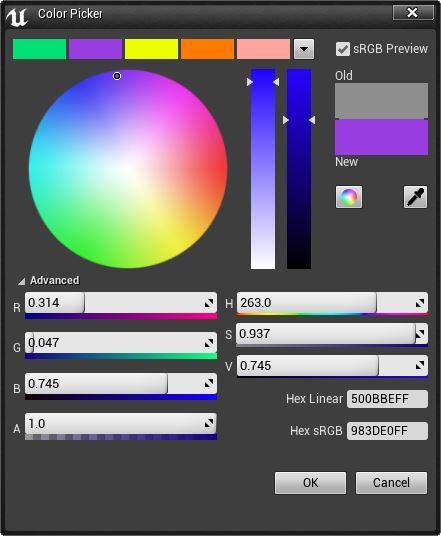
\includegraphics[width=.82\linewidth]{2dui.jpg}
  \caption{2D picker (UnrealEngine4 2012)}
\end{subfigure}%
\begin{subfigure}{.5\textwidth}
  \centering
  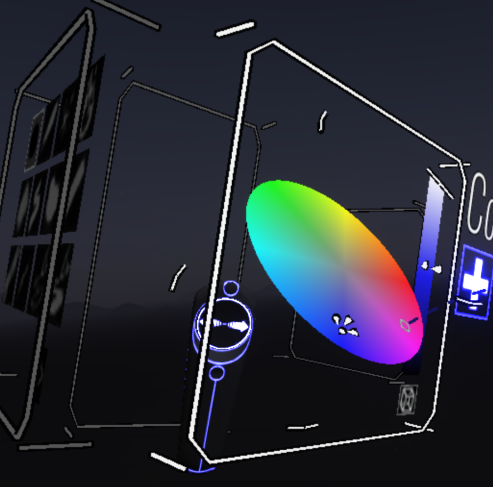
\includegraphics[width=1\linewidth]{3dui.png}
  \caption{3D colour picker (Tilt Brush 2016)}
\end{subfigure}
\caption{Comparison between 2D and 3D interface}
\end{figure*}

These features combined provide a sense of immersion or 'presence' not available using traditional 2D monitors. On the horizon is the next step in immersive technology, augmented reality (AR). This will allow a wireless experience and build upon the work in mobile virtual reality by Google and Samsung. Microsoft's Hololens provides a glimpse at this future, one of seamless multi-user interaction overlaid onto reality.

Current virtual reality interfaces tend to focus on using handheld virtual objects for natural interaction, a pen to draw on a surface or a handle to open a drawer. Issues arise in these interfaces when the objects or elements are not within reach. A common solution is a 3D pointer used to select distant items but for smaller targets or complex scenarios, pointers can be imprecise and slow to use (Malaika 2015). This project will look at how the usability of interfaces in VR can benefit from being dynamic and adaptive. It will reference concepts and techniques such as gaze-based interaction, error analysis and user modelling explored previously by other researchers in 2D and 3D. Figure 1 shows a comparison between a 2D and 3D interface.

\textbf{Research Question:} \\
''How can complex virtual reality interfaces be made more usable by employing adaptive user interface techniques?''

\textbf{Aims:}
\begin{itemize}[noitemsep,topsep=0pt]
\item Create iterations of a complex 3D interface for virtual reality, employing several adaptive user interface techniques.
\item Use quantitative data gathered from error analysis to assess any benefits to usability the adaptive techniques have.
\item Use qualitative data gathered from surveys to evaluate the overall effect of adaptive user interfaces on usability.
\end{itemize}
\textbf{Objectives:}
\begin{itemize}[noitemsep,topsep=0pt]
\item Research adaptive user interface techniques for 2D and 3D interfaces.
\item Implement a complex 3D user interface for use in virtual reality.
\item Employ the researched techniques for assessment.
\item Create a system for error analysis to gather qualitative evaluation data.
\item Have users test the iterations of the interface and feedback on their usability.
\item Compare the various techniques using the qualitative and quantitative data gathered to evaluate their effectiveness.
\item Using the comparisons evaluate the overall impact of adaptive user interfaces on usability in virtual reality.
\end{itemize}

\section{Context}
\subsection{Adaptive User Interfaces}
Dynamic user interfaces fall under a few categories in the area of research sometimes referred to as 'interface plasticity'. ‘A survey of plasticity in 3D user interfaces' (Jeremy 2014) gives an overview of the different types of dynamic user interface classifying them using two parameters, the adaptation time and the controller. Within these parameters an adaptive user interface is defined as being adapted by the system at run-time. This project will focus on implementing systems that fall under this classification of adaptation.

Many researchers have explored various ways to assist the user in digital environments since the early days of personal computing (Morgan 1998). One strategy known as intelligent user interfaces, seeks to actively learn how a user interacts with an interface and suggest or highlight relevant information accordingly. Although this can be effective, it takes time to model the user in a meaningful way and can seem obstructive as demonstrated by Microsoft's Clippy (Meyer 2015).

Another approach, the one this project focuses on, is to adapt the interface itself in direct response to the user's actions. One of these techniques covered by 'Modeling error-based Adaptive User Interfaces' (Kathik 2011) monitors the user's failures while navigating and interacting with an application to dynamically improve the interface. 'Adaptive Hypermedia and Adaptive Web-Based Systems' (Peter 2000) discusses the benefits of adapting a 3D environment as the user interacts with it to assist their actions.

Most user interfaces in our digital lives are static with adaptive interfaces reserved for improving accessibility for atypical users or use-cases. VR provides a new platform for innovation and does not have a counterpart to the universal language of 2D interfaces' windows and pointers. This uncharted territory provides an opportunity to experiment with dynamic 3D interfaces in new ways.

\subsection{Usability in Virtual Reality}
The companies and developers at the forefront of the new wave of virtual reality hardware and software have faced many challenges in comfort and usability. Issues with nausea and motion sickness plagued early iterations of head mounted displays. The addition of positional tracking and a greater understanding of significant design choices like locomotion have overcome most of these growing pains.

Now the focus of research is around usability of interfaces in VR. Valve, a driving force in desktop VR, presented some factors of usability at the Game Developer's Conference. When discussing interactions outside the user's area of reach they cited Fitt's law (Malaika 2015). This law has been extended from one dimensional interfaces into 2D interfaces and now into 3D and states that the speed at which a user acquires a target is exponentially proportionate to the size of the target at a given distance (Atsuo 2001). When using a pointer based system, small interface elements at a distance away become very slow to interact with. 

Another notable aspect of ease-of-use regards the placement of interface elements around the user. Due to the 360 degree nature of a 3D interface if the user is constantly required to turn around in order to perform actions it will become fatiguing. Owlchemy labs, developers of Job Simulator and strong proponents of diegetic interfaces build scenarios in such a way that users do not have to turn frequently and generally have direct access to everything they may need at a given time (Schwartz 2015).

\section{Methodology}
\subsection{Overview}
A template interface will be created to allow iteration using various adaptive techniques. This interface will be in a draft state with the first technique for the feasibility demo due at the end of first semester. The first weeks of second semester will be spent implementing the various other adaptive techniques researched and ensuring the interface is complex enough to create an environment in which usability becomes a noticeable factor to the user. \emph{Figure 2} shows a more detailed breakdown of the project timeline. The application interface will consist of an introduction during which the user will learn the basic interaction with the motion controllers and the basic navigation tools along with the function of the interface they are using.

\begin{figure*}
\centering
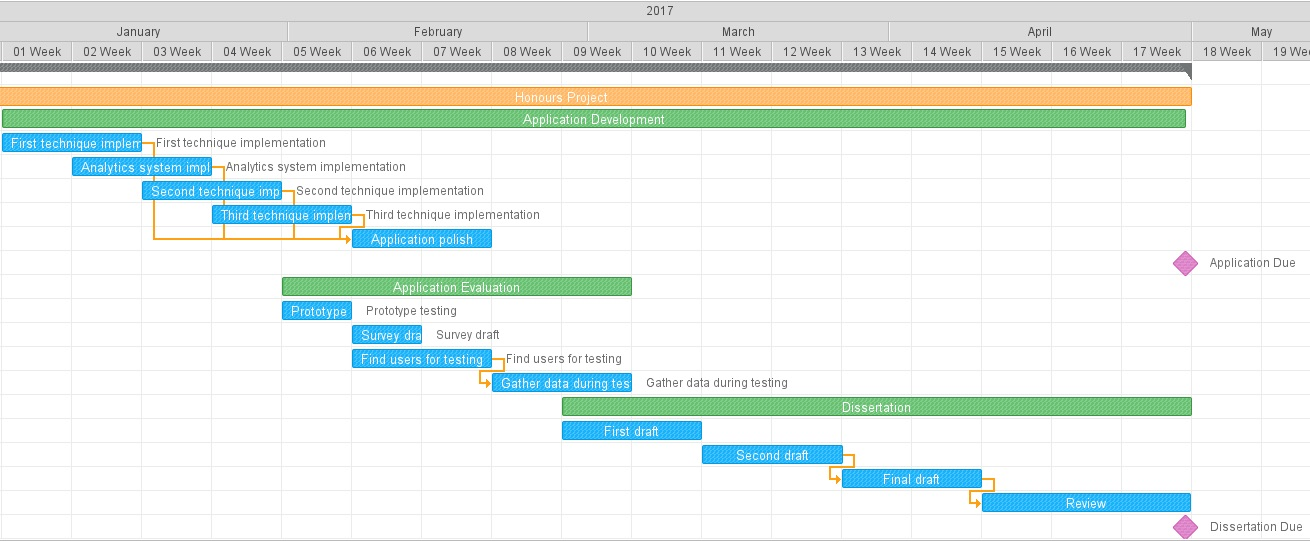
\includegraphics[width=1.\linewidth]{schedule}
\caption{Project Timeline}
\end{figure*}

\subsection{Implementation}
The interface will require the user to interact with various objects at different locations and distances away from them with complexity added by grouping and size of the elements. These interactions revolve around the 3 of the '5 universal interactions of 3D interfaces', namely: navigation, selection and manipulation (Bye 2016). The static version will require the user to precisely select and perform each action while the adaptive iterations will assist the user as they interact. Ideally every adaptive technique would be implemented and assessed but to manage the timescale of the development period before testing three adaptive techniques will be used initially.

The first will utilise basic analysis of errors made by the user, this would attempt to recognise missed clicks, reversals and general failure to use the interface. A reversal occurs when the user tries to immediately undo an action. Based on the context of an error the system will interpret the user's intended action and execute, highlight or suggest so as to avoid the user repeating an error. The system for recognising errors will be used in conjunction with other techniques in order to gather data about how usable the interface is.

Another implementation will use some form of pattern recognition. An example would be to build Markov chains representing common sequences of user actions, which the system can then reference to give the user suggestions. One risk associated with adaptive techniques is that new users learning an interface may have trouble when the system is trying constantly to assist them. The final technique researched is gaze-based interaction. This involves the system tracking objects the user may be focusing on and assisting interactions with that object if it is out of reach.

The implementation of the application and interfaces will use C++ within Unreal Engine 4. This handles rendering and projection for virtual reality as well as tracking of the headset/controllers, allowing the project to focus on the implementation of adaptive techniques. Simple graphics and 3D primitives will be used for visualisation in order to ensure the interface is the primary concern of the user as opposed to the assets and scene. The application should be device agnostic as Unreal Engine 4 supports each of the headsets and controllers, however if there are problems only one will be catered for and tested with. 

\subsection{Evaluation}
After the application has been implemented the evaluation of the interfaces will take place. Users will be gathered and surveyed through both the error analysis and feedback forms. There are also some existing analytics systems for VR that have been researched (Merki 2016), but a simpler focused custom system will be used in the project. This data will then be used to evaluate the effectiveness of each individual technique and the overall impact of adaptive interfaces for virtual reality. The usability survey given to each tester will break down into several short sections borrowing from 'Applying Usability Heuristics to VR' (Jen 2016). The speed at which they felt they were able to interact, the number of errors they made during interactions and the general intuitiveness of the application or any adaptive techniques used.

Using the qualitative and quantitative data gathered during the testing various representations of the user experience will be generated. Simple graphing of interactions and errors against time will hopefully demonstrate certain correlations. It is expected that all users will gradually become faster at performing interactions as they learn the interface and this will need to be accounted for when determining the experience of the adaptive interface versus the static interface. By comparing these graphs against the user's evaluation of their experience it will give an idea of how many errors a user makes before becoming frustrated, again this will be affected by the learning experience and the personality of the user. 

There may be other points of interest revealed by the data such as one error leading to a chain of errors or an error leading to a slow down in interaction time. All of these factors will help determine the effectiveness of the adaptive elements. If a user performs fewer errors in the adaptive system than in the static interface the qualitative data should support that the user experience was better in general.

\section{Summary}
The use of adaptive user interfaces should provide benefits to the usability of the 3D interfaces as well as the speed at which the user can interact with them. This will allow for more complex interfaces capable of performing more meaningful and productive tasks. With a future that could be rooted in virtual reality, it is the opportune time to re-evaluate what an interface can be and how the system reacts to the user. With the promise of wireless headsets and augmented reality on the horizon, traditional 2D displays could quickly become obsolete. If our walls, floor and hands can be our displays then the interfaces will need to become more dynamic and versatile. Adaptive user interfaces have been researched for a long time and could soon become essential to our everyday interactions.

Improving upon the language of 2D interfaces will be a huge challenge as they are so deeply engrained in our digital lives. The transition so far has been fairly slow with the majority of virtual reality interfaces using 2D elements in 3D space or 3D objects that mirror those in reality. The interesting interfaces will hopefully begin to emerge as more abstract interactions emerge. The first of these is beginning to trickle through in the likes of Fantastic Contraption which asks you to put on a space helmet to access the menu environment (Northway 2016). The evolution of virtual reality and augmented reality will depend on developers detaching themselves from our preconceptions about what an interface can be and embracing concepts like adaptivity.

\pagebreak

\section{References}
Anastasios, K. 2012. \emph{When You Shouldn't Use Fitts's Law To Measure User Experience} Smashing. 

Atsuo, M. 2001. \emph{Extending Fitts' law to a three-dimensional pointing task} Japan. Elsevier. 

Brusilovsky, P. 2000. \emph{Adaptive Hypermedia and Adaptive Web-Based Systems} Italy. Springer.

Bye, K. 2016. \emph{Five Universal Tasks of 3D User Interfaces with Doug Bowman} Voices of VR. Available at: \url{http://voicesofvr.com/five-universal-tasks-of-3d-user-interfaces-with-doug-bowman/} [Accessed November 2016]

Jen, H. 2016. \emph{Designing for VR: Applying Usability Heuristics to Virtual Reality} Omobono. 

Jeremy, L. 2014. \emph{A survey of plasticity in 3D user interfaces} Minneapolis. IEEE. 

Karthik, R. 2011. \emph{Modeling error-based Adaptive User Interfaces} Iowa State University. 

Malaika, Y. 2015. \emph{Interaction Design in VR: Valve's Lessons } Available from: \url{https://www.youtube.com/watch?v=_vQo0ApkAtI} [Accessed October 2016]

Merki, R. 2016. \emph{How VR Analytics Makes Your Product Better} Available from: \url{http://cognitivevr.co/blog/how-vr-analytics-makes-your-product-better/} [Accessed October 2016]

Meyer, R. 2015 \emph{Even Early Focus Groups Hated Clippy} Available from: \url{http://www.theatlantic.com/technology/archive/2015/06/clippy-the-microsoft-office-assistant-is-the-patriarchys-fault/396653/} [Accessed October 2016]

Morgan, K. 1998. \emph{Intelligent User Interfaces: An Introduction} San Fransisco. RUIU 

Northway, C. 2016. \emph{Menus Suck} VRDC. Available at: \url{http://www.gdcvault.com/play/1023668/Menus} [Accessed November 2016]

Pino, N. 2016 \emph{HTC Vive review} Available from: \url{http://www.techradar.com/reviews/wearables/htc-vive-1286775/review/3} [Accessed October 2016]

Robert, Z. \emph{Look-That-There: Exploiting Gaze in Virtual Reality Interactions} Providence. Brown University. 

Schwartz, A. 2015. \emph{Being There: Designing Standing VR Experiences with Tracked Controllers} Available from: \url{https://www.youtube.com/watch?v=hjc7AJwZ4DI} [Accessed October 2016]
	
Seeto, D. 2016 \emph{Gamestop: PSVR Exceeding Expectations As More Units Are Received For Holiday Season} Online. \url{http://attackofthefanboy.com/news/gamestop-playstation-vr-exceeding-expectations-units-received-holiday-season/} [Accessed October 2016]

\emph{Tilt Brush.} 2016. [software]. HTC Vive. Google. 

\emph{Unreal Engine 4.} 2012. [software]. Windows. Epic Games. 


\section{Bibliography}
Alger, M. 2015. \emph{VR Interface Design Manifesto} Available from: \url{https://www.youtube.com/watch?v=n3b8hZ5NV2E} [Accessed October 2016]

Casey, H. 2015. \emph{Designing For Virtual Reality} Online. UsTwo. [Accessed October 2016]

Julie, J. 2011. \emph{Human-Computer Interaction} 2011. Springer. 

Max, G. \emph{The UX of VR} Available from: \url{http://www.uxofvr.com/} [Accessed October 2016]

Nasoz, F. 2004. \emph{Adaptive Intelligent User Interfaces with Emotion Recognition} Orlando State University. 

Rhino, K. 2016. \emph{Building 3-Dimensional UI for VR} Available from: \url{http://www.gdcvault.com/play/1023652/Building-3-Dimensional-UI-for-VR} [Accessed October 2016]

Shaw, C. \emph{Pain and Fatigue in Desktop VR: Initial Results} Canada. University of Regina. 

Stanney, K. 1998. \emph{Human Factors Issues in Virtual Environments: A Review of the Literature} Orlando. MIT. 

Sutcliffe, A.G. \emph{A Usability Evaluation Method for Virtual Reality User Interfaces} Manchester. UMIST. 

Viano, G. 2000. \emph{Adaptive User Interface for Process Control based on Multi-Agent approach} Italy. ACM. 

\end{document}

